\documentclass[a4paper]{article}

\usepackage{times}
\usepackage{tikz}
\usepackage[margin=0cm]{geometry}
\usepackage{graphicx}
\usepackage{anyfontsize}
\usepackage{fancyhdr}
\usepackage{indentfirst}
\usepackage{amsmath}
\usepackage[spanish]{babel}
\usepackage[utf8]{inputenc}
\usepackage{titlesec}
\usepackage{enumitem}
\usepackage{caption}

\author{}
\date{}
\title{}

\begin{document}
\thispagestyle{empty}

\begin{tikzpicture}[remember picture, overlay]
    \pgftransformshift{\pgfpoint{0cm}{0cm}}
    \draw [line width=2pt](1cm,-1cm) -- (1cm,-27.7cm) -- (14cm, -27.7cm) -- (14cm, -1cm) -- (1cm, -1cm);
    \draw[line width=2pt] (15cm, -27.7cm) -- (19cm,-27.7cm) -- (19cm, -1cm) -- (15cm, -1cm) --  (15cm, -27.7cm);
    \node [line width=2pt] at (17cm, -3.5cm) {
\includegraphics[width=3cm]{../imagenes/utn.png}};
		\node [line width=2pt] at (7.5cm, -7.5cm) {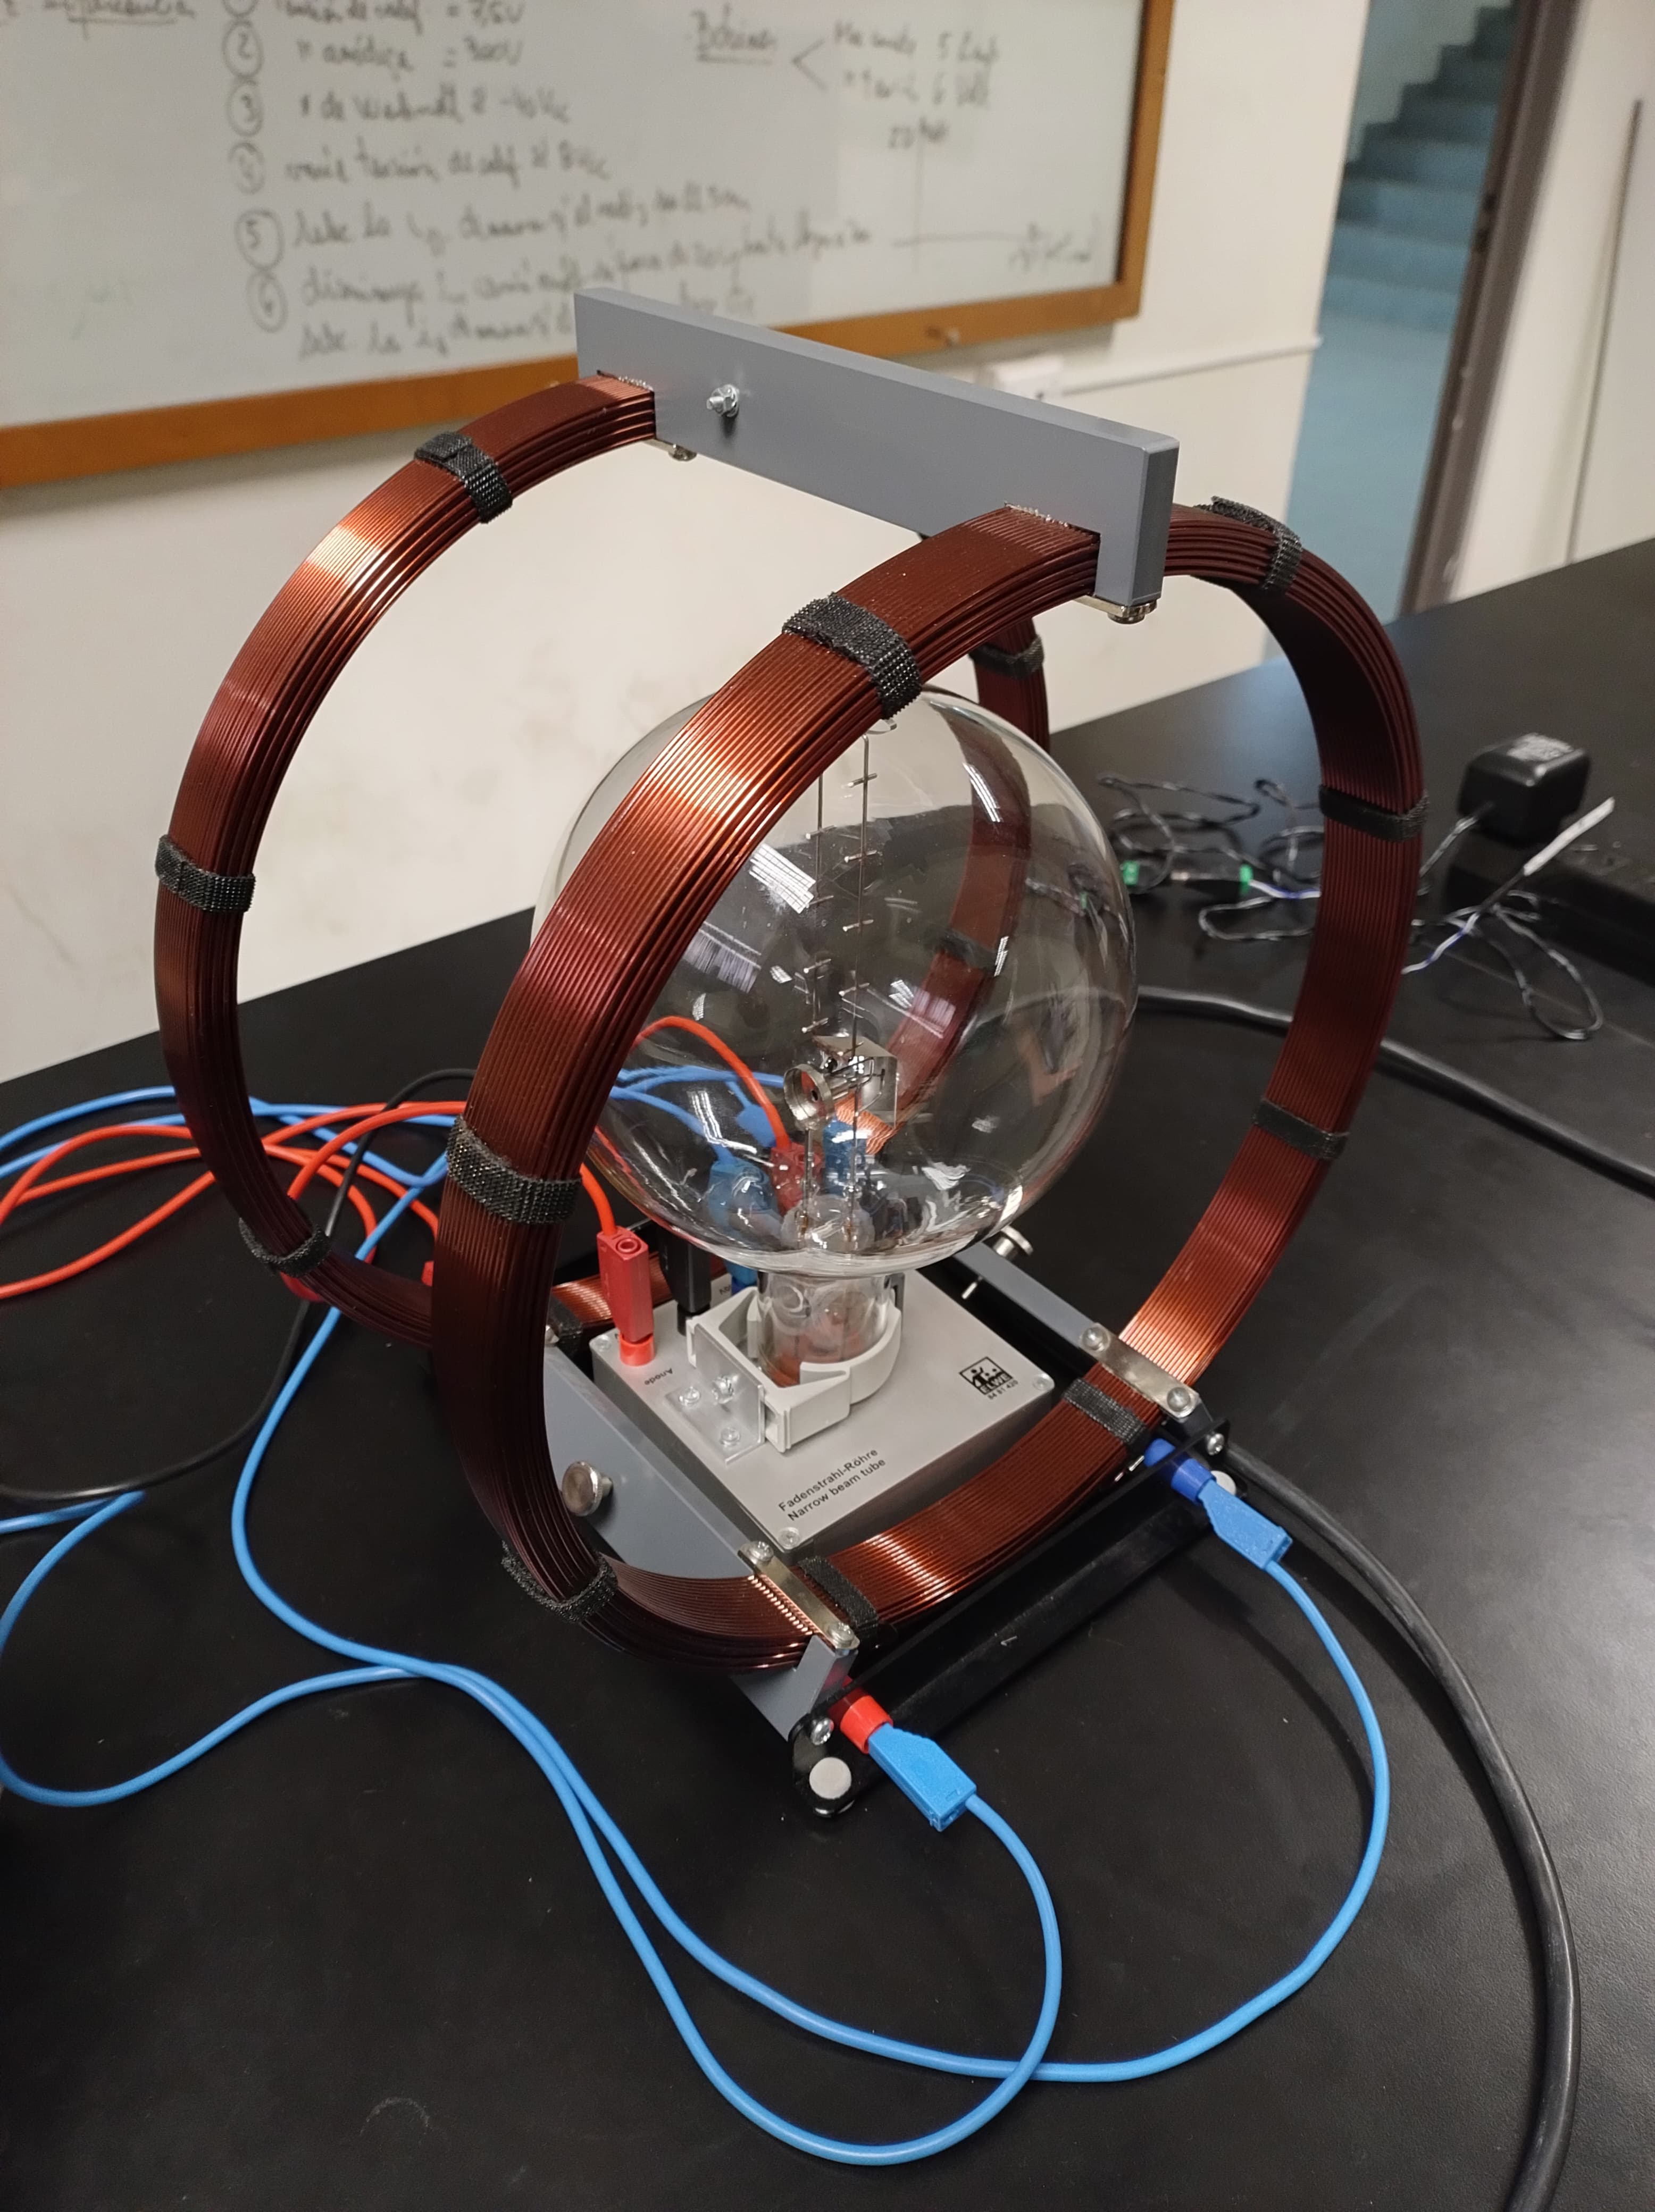
\includegraphics[width=6cm]{../imagenes/ampollaYBobinasHelmholtz.jpeg}};
    \node at (17cm, -7cm) {\scalebox{5}{\textbf{U}}};
    \node at (17cm, -9cm) {\scalebox{5}{\textbf{T}}};
    \node at (17cm, -11cm) {\scalebox{5}{\textbf{N}}};
    \node at (17cm, -14cm) {\scalebox{5}{\textbf{F}}};
    \node at (17cm, -16cm) {\scalebox{5}{\textbf{R}}};
    \node at (17cm, -18cm) {\scalebox{5}{\textbf{C}}};
    \node at (7.5cm, -13cm) {\scalebox{2.5}{\textbf{Carga específica}}};
    \node at (7.5cm, -14cm) {\scalebox{2.5} {\textbf{del electrón}}};

    \node at (7.5cm, -22cm) {
        \begin{minipage}[c]{12cm}
            \begin{itemize}
                \raggedright
                \vspace{1.5cm}
                \item \fontsize{12}{12}\selectfont \textbf{Autores:} \vspace {1mm} \fontsize{11}{12}\selectfont \\
                    \begin{itemize}
                        \item \hspace{2mm} Valentino Rao - Leg. 402308 \\
                        \item \hspace{2mm} Ignacio Ismael Perea - Leg. 406265 \\
                        \item \hspace{2mm} Manuel Leon Parfait - Leg. 406599 \\ 
                        \item \hspace{2mm} Gonzalo Filsinger - Leg. 400460 \\ 
                        \item \hspace{2mm} Agustín Coronel - Leg. 402010 \\
                        \item \hspace{2mm} Marcos Raúl Gatica - Leg. 402006 \\
                    \end{itemize}

                \item \fontsize{12}{12}\selectfont \textbf{Curso:} 2R1. \\
                \item \fontsize{12}{12}\selectfont \textbf{Asignatura:} Física electrónica. \\
                \item \fontsize{12}{12}\selectfont \textbf{Institución:} Universidad Tecnológica Nacional - Facultad Regional de Córdoba \\

            \end{itemize}
        \end{minipage}};

\end{tikzpicture}

\renewcommand{\normalsize}{\fontsize{12}{18}\selectfont}
\newgeometry{margin=1cm}
\fancyhf{}
\renewcommand{\headrulewidth}{0pt}
\renewcommand{\footrulewidth}{0pt}
\fancyfoot[R]{[Rao V. - Parfait M. - Filsinger G. - Perea I. - Coronel A - Gatica M.] [\textbf{pág. \thepage}]}
\setlength{\footskip}{0pt}
\newpage
\thispagestyle{empty}
\text{}

\titleformat{\section} {\fontsize{12}{12}\bfseries}{\thesection.}{0.5em}{\underline}

\newpage
\newpage

\thispagestyle{empty}
\setcounter{page}{0}
\tableofcontents

\newpage
\thispagestyle{fancy}
\twocolumn
\flushbottom
\section{INTRODUCCIÓN}

    \indent El objetivo de este informe es detallar la experiencia de laboratorio llevado a cabo para la medición de la carga específica del electrón, utilizando un dispositivo compuesto por: \\

    \begin{enumerate}
        \item Un tubo de rayos filiformes que generan los electrones y los acelera bajo la acción de una diferencia de potencial. 
        \item Un par de bobinas de Helmholtz encargadas de generar un campo magnético uniforme entrante, encargado de someter a los electrones. 
    \end{enumerate}

    \begin{figure}[h!]
        \centering
        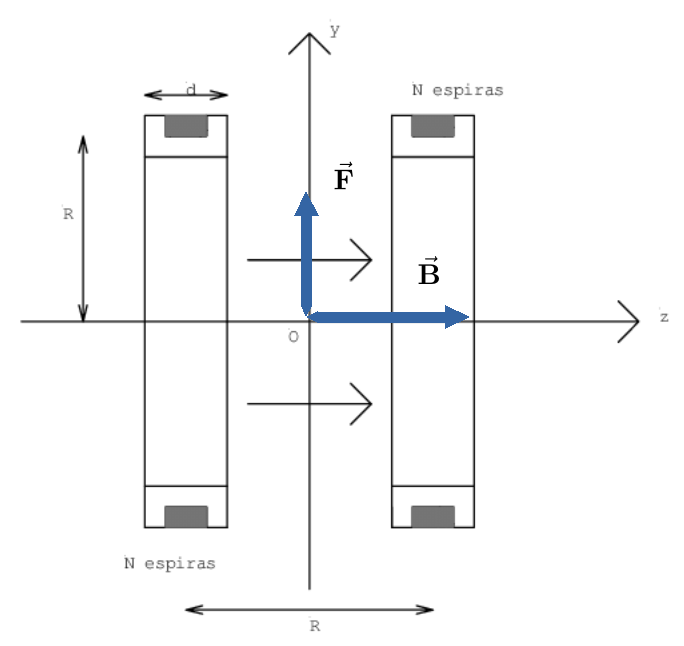
\includegraphics[width = 7.5cm] {../imagenes/dibujoBobinasHelmholtz.png}
    \end{figure}

    \begin{center}
        \textit{Vista lateral izquierda de las bobinas Helmholtz.}
    \end{center}

    \subsection{Fundamentos teóricos}
    \indent La fuerza de Lorentz que afecta al electrón entre cátodo y ánodo, perpendicular al campo $\vec{B}$ generado por las bobinas de Helmholtz y perpendicular a la velocidad, es dada por:

    \begin{center}
        $\vec{F} = e (\vec{v} x \vec{B})$ 
    \end{center}

    \indent Esta fuerza provoca que el electrón adopte una trayectoria orbital, con un cierto radio. \\
    \indent Esto se puede relacionar con la expresión de una fuerza centrípeta que actúa sobre un cuerpo con masa que describe una circunferencia:

    \begin{center}
        $\vec{F} = m {\frac {(\vec{v})^2}{r}}$
    \end{center}

    \indent Ambas expresiones de fuerza son iguales, por lo tanto se puede decir que:

    \begin{center}
        $e \vec{v} \vec{B} = m {\frac {(\vec{v})^2}{r}}$
    \end{center}

\end{document}
